\documentclass[12pt]{article}

\usepackage[english]{babel}

% Math/Greek packages
\usepackage{amssymb,amsmath,amsthm, mathtools} 
\usepackage{algorithm, algorithmic}
\usepackage{upgreek, siunitx}

% Graphics/Presentation packages
\usepackage{geometry, graphicx, subcaption}
\usepackage{tabulary, enumitem, array}
\usepackage{xparse,mleftright,tikz}
\usepackage{physics}

% Misc packages
\usepackage{fancyhdr}


\usepackage[export]{adjustbox}

\usepackage{esint}

\sisetup{locale=US,group-separator = {,}}
\usepackage[colorlinks=true, allcolors=blue]{hyperref}


% Box function - update this as more sophisticated solutions are found
\newcommand\mybox[2][]{\tikz[overlay]\node[fill=blue!20,inner sep=2pt, anchor=text, rectangle, rounded corners=1mm,#1] {#2};\phantom{#2}}
\renewcommand{\arraystretch}{1.2}

% General macro declarations


\makeatletter
\let\oldabs\abs
\def\abs{\@ifstar{\oldabs}{\oldabs*}}
%
\let\oldnorm\norm
\def\norm{\@ifstar{\oldnorm}{\oldnorm*}}
\makeatother

\begin{document}

\title{PHSX 491: HW01 - Mass Equivalence}
\author{William Jardee}
\maketitle


\section*{Question 1}
{\sl Here we will work to convince ourselves that the inertial mass and gravitational mass are indeed equivalent. Consider two objects, one near the surface of the Earth and the other out in deep space where it cannot interact with any other objects. Each object has teh same inertial mass $m_i$ and gravitational mass $m_g$. For simplicity we will take the speed of light to one, $c \rightarrow 1$.}

\begin{enumerate}[label=\alph*)]
\begin{figure}[!ht]
\centering
	\begin{subfigure}{0.45\textwidth}
	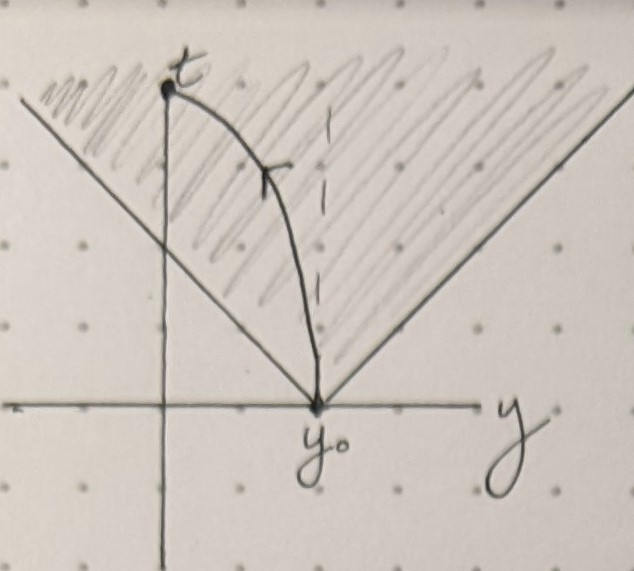
\includegraphics[width=\textwidth]{gr_1.1.jpg}
	\caption{The 2-dimensional spacetime diagram for part's {\bf a)} and {\bf b)}. The shaded region is the ``light cone", those are the points that are said to be time-like (aka, they could be related by two event separated in time).}
	\label{fig:1.1}
	\end{subfigure}
	\hfill
	\begin{subfigure}{0.45\textwidth}
	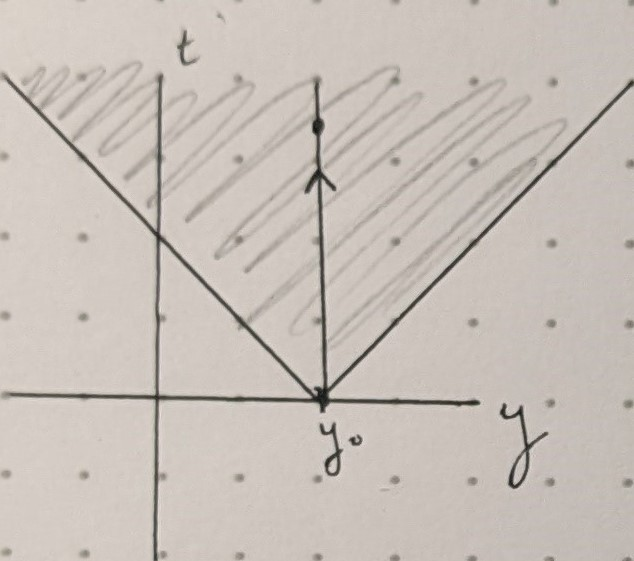
\includegraphics[width=\textwidth]{gr_1.2.jpg}
	\caption{Yeah, not gonna explain this for all of them. This is for {\bf c)}}
	\label{fig:1.2}
	\end{subfigure}
\end{figure}

\item {\sl Barrett's questions are quite wordy, so I'm just gonna skip copying it all down... if I feel like it is needed to track the question I will quote it, otherwise I will assume that you know these questions intimately enough...}\\

See Fig.~\ref{fig:1.1}

\item See Fig.~\ref{fig:1.1} \\
Isn't this just so exciting! Considering all of this is physics that we have been doing for numerous years, I assume that I don't need to elaborate any more on how to do a simple ``$ct \times x$" diagram. 

\item See Fig.~\ref{fig:1.2} \\ In this case, the path is not a geodesic. Our working definition of geodesic is the `shortest path that connects two points in spacetime.' Pairing this with the Geodesic Hypothesis that `A free particle will move along a geodesic', since this particle is no longer a free particle (we are exerting a force on it) the path it follows can't be the geodesic in spacetime.

\item The force of gravity is seen in Fig.~\ref{fig:1.1} is going to be the particle's response to the gravitational field:
\[F_g = \frac{GM}{r^2}m_G = g \cdot m_G\]
Where we are calling 
\[g = \frac{GM}{r^2}\]
Thus, the upwards force must be
\begin{equation}
F_g^\prime = - g \cdot m_G
\label{eq:1}
\end{equation}


\begin{figure}[!ht]
\centering
	\begin{subfigure}{0.45\textwidth}
	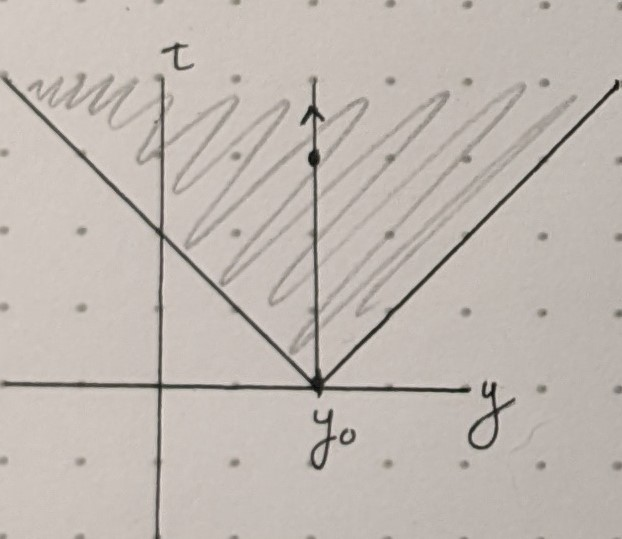
\includegraphics[width=\textwidth]{gr_1.3.jpg}
	\caption{You know the drill: {\bf e)} and {\bf f)}}
	\label{fig:1.3}
	\end{subfigure}
	\hfill
	\begin{subfigure}{0.45\textwidth}
	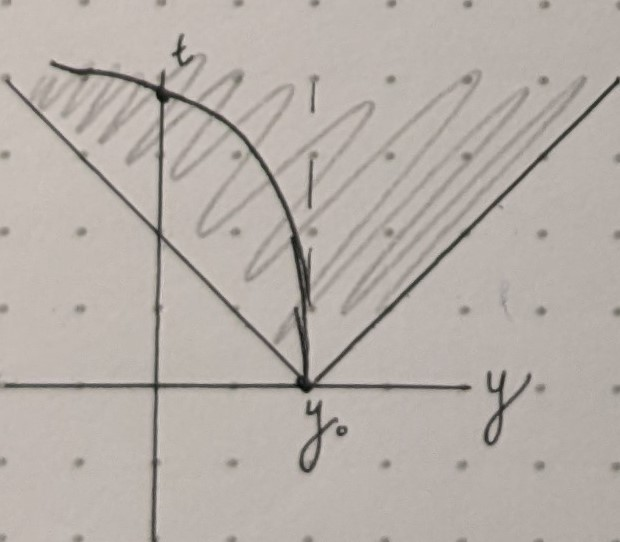
\includegraphics[width=\textwidth]{gr_1.4.jpg}
	\caption{Bro, have you ever tried soy sauce in mac \& cheese? It is surprisingly good. You should try it sometime - just don't over do it on the salt when you're making the pasta... Oh, and: {\bf g)}}
	\label{fig:1.4}
	\end{subfigure}
\end{figure}

\item See Fig.~\ref{fig:1.3}

\item See Fig.~\ref{fig:1.3}

\item See Fig.~\ref{fig:1.4}\\
Very similar to the answer in part {\bf c)}, this path will not be the geodesic since the path being follow is not being done by a free particle. I will also drop this here to have for the next part: The force must be:
\begin{equation}
F_I = g \cdot m_I
\label{eq:2}
\end{equation}


\item Looking at Fig~\ref{fig:1.1} and Fig.~\ref{fig:1.4}, intuition says that their paths are the same. To justify that statement, we can simply say that the acceleration both of them see must be the same (as that was given in part {\bf g)}). Since both have the same initial conditions and equations of motions, by uniqueness of solutions, their curves must be identical. So, assuming there is a unique way to transform a trajectory (which is a reasonable assumption, but this last week has kinda messed with some of my assumptions recently, so who knows.), then their forces must be equivalent. 

\item In part {\bf h)} we said that Eq.~\ref{eq:1} and Eq.~\ref{eq:2} must equal\footnote{That is in magnitude, their directions will be opposite because of the way I defined the forces.}, so:
\[-F_G = F_I\]
\[g \cdot m_G = g \cdot m_I\]
\[\boxed{m_G = m_I}\]

\end{enumerate}

\end{document}